Met alle elementen op het scherm kan je de searchbar gebruiken om te zoeken op applicaties en bestanden. Als je zoekt op
Word, een Microsoft applicatie die niet op Linux beschikbaar is, dan vind je LibreOffice Writer een gratis en open
source alternatief. Start de applicatie op.

{\selectlanguage{dutch}
Neem de tekst over van het plaatje hierboven en zorg dat dit een eerste hoofdstuk titel wordt door de stijl te
veranderen. We gaan het document later vullen. Selecteer File en Save as{\dots} om het bestand op te slaan als
Document1.}

\begin{figure}[H]
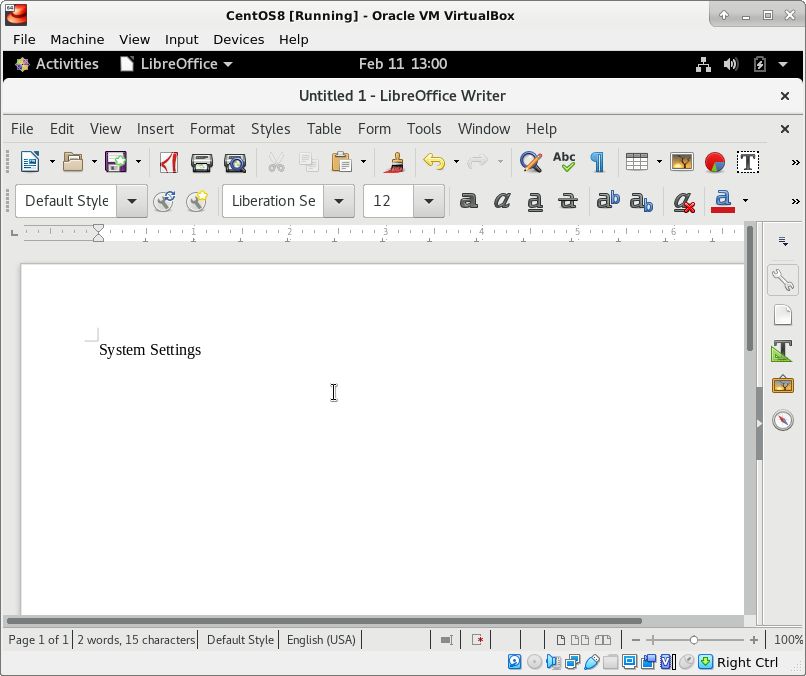
\includegraphics[width=0.9\textwidth]{linuxreader-img015.png}
\end{figure}
{\selectlanguage{dutch}
\foreignlanguage{dutch}{Meer over LibreOffice en de verschillende onderdelen van dit office pakket komt later aan de
orde als we Office Pakketten gaan bespreken. Nu concentreren we ons eerst op de beschikbare scherm elementen.}}
